\chapter{Einleitung}

Das Reinforcement-Lernen (RL) kann als zielorientierte Interaktion eines lernenden Subjekts mit seiner Umgebung beschrieben werden. Zusammen mit dem überwachten und unüberwachten Lernen bildet es die drei großen Paradigmen des maschinellen Lernens. Während bei den beiden Erstgenannten für gewöhnlich ein feststehender Datensatz die Basis des Lernprozesses bildet, gibt es diesen im RL nicht. Stattdessen wird durch die Interaktion mit der Umgebung gelernt. Ebendiese Interaktion besteht aus der Auswahl von Aktionen, basierend auf Beobachtungen der Umgebung, die wiederum die getätigten Aktionen wahlweise belohnt oder bestraft. Mittels RL konnten in den vergangenen Jahren verschiedenste Problemstellungen erfolgreich gelöst werden. Diese erstrecken sich über Themen der Robotik \cite{MappingPlanning}, über das Spielen von Brettspielen wie Go \cite{Go}, bis hin zum Lösen algorithmischer Probleme \cite{DNC}. In vielen Bereichen konnten die Ergebnisse mittels RL wahlweise signifikant verbessert oder überhaupt erst ermöglicht werden. Aufgrund der vielfältigen Einsatzmöglichkeiten und erzielten Resultate ist das RL ein Thema von großem Interesse in der aktuellen Forschung im Bereich des maschinellen Lernens.

Im Kontext von Navigationsproblemen ist es nicht möglich, lediglich auf Basis der aktuellen Beobachtung sinnvoll zu handeln, da diese wiederum nur einen kleinen Ausschnitt der Umgebung beinhaltet. Vielmehr wird auch Wissen darüber benötigt, was schon gesehen wurde bzw. nicht gesehen wurde. Dies ist unabdingbar, um die Umgebung effizient zu erkunden und eine zielgerichtete Navigation zu vollziehen. Es wird demnach eine Art Gedächtnis benötigt. Dieses ist beim Navigieren idealerweise in Form einer Karte aufgebaut, d.h. es verfügt über eine räumliche Struktur. Die Karte sollte mit jeder aktuellen Observation Stück für Stück erweitert werden, sodass alle vergangenen Observationen in ihr enthalten sind. Darüber hinaus sollte das lernende Subjekt, welches im RL Kontext üblicherweise als Agent bezeichnet wird, die Karte auch gewinnbringend für die Auswahl seiner Aktionen einsetzen können. Ein vielversprechender Ansatz in diesem Zusammenhang ist die von Parisotto und Salakhutdinov präsentierte Neural Map \cite{NeuralMap}. Hierbei handelt es sich um ein voll differenzierbares Modell für einen RL Agenten. Somit können seine Parameter mit einem Gradientenabstieg erlernt werden. Insbesondere verfügt das Modell über einen trainierbaren Lese- ud Schreiboperator. Der Leseoperator ermöglicht es, die Karte im Speicher des Modells abzufragen auf Basis der aktuellen Beobachtung. Somit kann überprüft werden, ob der Agent etwas Ähnliches bereits gesehen hat oder nicht. Da der Operator trainierbar ist, kann er erlernen, was im Kontext der Problemstellung als ähnlich angesehen werden kann. Der Schreiboperator wiederum kann erlernen, was bezüglich der Aufgabe des Agenten relevant ist und somit in den Speicher geschrieben wird. Auf diese Weise ermöglichen die beiden Operatoren, sowohl die Generierung als auch die Nutzung der Karte zu erlernen.

Dabei beschreibt der Schreiboperator in einem Schritt bzw. einem Update jedoch nur eine Speicherposition, die wiederum der aktuellen Position des Agenten entspricht. Dies ist eine Limitierung der Neural Map. Oftmals enthält die Beobachtung des Agenten relevante Informationen der Umgebung, die jedoch räumlich gesehen in einer gewissen Entfernung zum Agenten liegen. So kann der Agent beispielsweise beim Blick in einen Raum bereits einen für seine Aufgabe später benötigten Gegenstand erblicken. Nun wäre es ziemlich umständlich, wenn der Agent tatsächlich den Raum betreten und sich an die Position des Gegenstands begeben müsste, um ihn korrekt bzw. sinnvoll in der Karte abspeichern zu können. Um dieses Problem zu überkommen, wird im Rahmen dieser Arbeit eine Erweiterung des Schreiboperators entwickelt. Diese beschreibt eine zusätzliche Speicherposition und zwar in Blickrichtung des Agenten. Auf diese Weise soll der Speicher schneller und effizienter gefüllt werden, was zu einer schnelleren Erstellung der Karte der Umgebung führt. Dies wiederum soll das Explorationsverhalten des Agenten begünstigen, d.h. die Zeitdauer zur Erkundung der Umgebung verringern. Darüberhinaus wird der Speicher durch die Erweiterung des Schreiboperators öfter beschrieben bzw. aktualisiert. Dadurch sollen relevante Informationen der Umgebung mit einer größeren Wahrscheinlichkeit auch korrekt in der Karte abgebildet werden. Beide zuvor angesprochenen Verbesserungsaspekte haben das Potential, die Navigationsfähigkeiten der Neural Map positiv zu beeinflussen und im Idealfall somit auch die Gesamtleistungsfähigkeit zu steigern. Inwiefern dies der Fall ist, wird im Rahmen verschiedener Zielsuche-Szenarien ergründet. Dabei wird die Neural Map mit der Erweiterung des Schreiboperators zum einen mit der von Parisotto und Salakhutdinov vorgestellten Variante verglichen und zum anderen mit einem als Referenz gewählten LSTM. Außerdem wird ein seperater Speichertest durchgeführt, in dem die Fähigkeit der Neural Map zur Kartenerstellung bewertet wird.

Als nächstes werden in Kapitel \ref{chap_basics} die Grundlagen des RL, des verwendeten Lernalgorithmus und der Neural Map erklärt. Die technischen Details der Implementierung des Lernalgorithmus und der Neural Map befinden sich in Kapitel \ref{chap_impl}. Insbesondere wird in diesem Kapitel auch die im Rahmen dieser Arbeit entwickelte Erweiterung für den Schreiboperator präsentiert. Das Kapitel \ref{chap_exp} enthält die durchgeführten Experimente und präsentiert die dazugehörigen Ergebnisse. Die Diskussion Letzterer findet dann in Kapitel \ref{chap_disc} statt.

















\iffalse

% Kapazitätstrends und Limits in optischen Kommunikationsnetzen \cite{Essiambre2012}\\
% Über die Durchbrüche auf dem Gebiet der optischen Netze im Jahr 2012 gibt \cite{Essiambre2013} einen
% Überblick. Viel verspricht man sich durch räumliches Multiplexen; neben Modenmultiplex auch durch den
% Einsatz von Mehrkernfasern.


Optische Kommunikationsnetze bilden bis heute die unangefochtene Grundlage für die Übertragung großer Datenmengen über weite Strecken bei gleichzeitig geringer Latenz.
Damit ist die optische Übertragungstechnik die Grundlage moderner Kommunikationsnetze und insbesondere des Internets.
Erste kommerzielle optischen Übertragungssysteme stellten gerade einmal eine Übertragungskapazität von weniger als \SI{100}{\mega\bit\per\second} zur Verfügung.\par\medskip
Die durchschnittliche Last am deutschen Internetknoten DE-CIX ist in Abbildung \ref{fig:DE-CIX} dargestellt. Derzeit liegt diese bei über \SI{1,4}{\tera\bit\per\second}.

\begin{figure}[ht!]
 \centering
 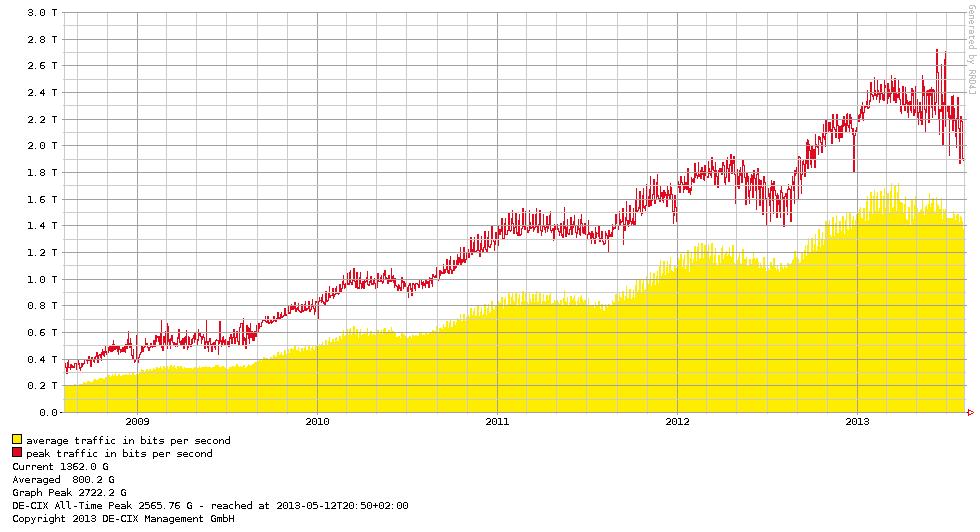
\includegraphics[keepaspectratio,width=0.9\textwidth]{abbildungen/de-cix_5y_20130804.png}
 \caption{DE-CIX Traffic Statistik, 5 Jahres Grafik \protect\footnotemark[1]}
 %\caption{DE-CIX traffic statistics, 5 year graph \protect\footnotemark[1]}
 \label{fig:DE-CIX}
\end{figure}

\footnotetext[1]{\url{http://www.de-cix.net/about/statistics/}}

Eine verständliche Einführung in die Tiefen der optischen Übertragungstechnik bietet das Vorlesungsskript OUET \cite{ouet}.
Eine weitere wichtigste Quellen ist \cite{Agrawal2012}.



\section{Abkürzungen}
Für Abkürzungen kann das Paket \textit{acronym} verwendet werden.
Ein Abkürzungsverzeichnis ist nicht erforderlich, sofern alle Akbürzungen bei der ersten Verwendung eingeführt werden.
Dies wird durch die Verwendung von \textit{acronym} vereinfacht, jedoch ist die Nutzung des Paketes rein optional.
Das Paket bietet folgende Optionen (siehe  \LaTeX~Quelltext):\par\medskip
\begin{itemize}
 \item \ac{NLSE}         % fügt die Abkürzung ein, außer beim ersten Aufruf, hier wird die Erklärung mit angefügt
 \item \acs{NLSE}        % fügt die Abkürzung ein
 \item \acf{NLSE}        % fügt die Abkürzung UND die Erklärung ein
 \item \acl{NLSE}        % fügt nur die Erklärung ein
\end{itemize}



\section{Mathematik}
Für mathematische Formeln wird das \textit{amsmath} Paket verwendet. Gleichungen sind damit recht schön zu setzen:

\begin{equation}
\frac{{\partial A}}{{\partial z}} =  - \frac{\alpha }{2}A + i{\beta ^{(0)}}A - {\beta ^{(1)}}\frac{{\partial A}}{{\partial t}} - i\frac{{{\beta ^{(2)}}}}{2}\frac{{{\partial ^2}A}}{{\partial {t^2}}} + i\gamma {\left| A \right|^2}A
\label{equ:nlse}
\end{equation}

Auch das Referenzieren von Gleichungen ist recht einfach. Dabei ist mit Gleichung \eqref{equ:nlse} eine mögliche Darstellungsform der \acs{NLSE} gegeben.

\fi
